\documentclass[11pt,a4paper,titlepage]{article}
\usepackage[utf8]{inputenc}
\usepackage[T1]{fontenc}
\usepackage[italian]{babel}
\usepackage{geometry}
\geometry{top=2.5cm,bottom=2.5cm,left=2.5cm,right=2.5cm}
\usepackage{amsmath,amssymb,amsfonts,amsthm}
\usepackage{graphicx}
\usepackage{xcolor}
\usepackage{tcolorbox}
\tcbuselibrary{skins,breakable}
\usepackage{listings}
\usepackage{booktabs}
\usepackage{tabularx}
\usepackage{fancyhdr}
\usepackage{titlesec}
\usepackage{enumitem}
\usepackage{hyperref}
\usepackage{microtype}
\usepackage{eurosym}

% --- Palette Colori Tecnico-Ingegneristica ---
\definecolor{techNavy}{HTML}{1A365D}
\definecolor{techBlue}{HTML}{2B6CB0}
\definecolor{techSlate}{HTML}{4A5568}
\definecolor{techLightBg}{HTML}{F7FAFC}
\definecolor{techBorder}{HTML}{CBD5E0}
\definecolor{techCodeBg}{HTML}{EDF2F7}
\definecolor{techGreen}{HTML}{22543D}
\definecolor{techRed}{HTML}{9B2C2C}

% --- Configurazione Hyperref ---
\hypersetup{
    colorlinks=true,
    linkcolor=techBlue,
    urlcolor=techBlue,
    citecolor=techGreen,
    filecolor=techNavy
}

% --- Configurazione Intestazioni e Pi\`e di Pagina ---
\pagestyle{fancy}
\fancyhf{}
\fancyhead[L]{\small\textbf{\color{techNavy}SIMO 2.0 Architecture Manual}}
\fancyhead[R]{\small\color{techSlate}\nouppercase{\leftmark}}
\fancyfoot[C]{\thepage}
\renewcommand{\headrulewidth}{0.5pt}
\renewcommand{\headrule}{\color{techBorder}\hrule width\headwidth height\headrulewidth \vskip-\headrulewidth}

% --- Configurazione Titoli di Sezione ---
\titleformat{\section}
  {\normalfont\Large\bfseries\color{techNavy}}{\thesection}{1em}{}[\color{techBorder}\titlerule]
\titleformat{\subsection}
  {\normalfont\large\bfseries\color{techBlue}}{\thesubsection}{1em}{}
\titleformat{\subsubsection}
  {\normalfont\normalsize\bfseries\color{techSlate}}{\thesubsubsection}{1em}{}

% --- Configurazione Listings per Codice Kotlin/SQL/JSON ---
\lstdefinelanguage{Kotlin}{
  keywords={package, import, class, object, interface, fun, val, var, data, sealed, override, companion, private, public, protected, suspend, return, if, else, when, while, for, in, is, null, true, false, try, catch, finally, throw, this, super, by},
  keywordstyle=\color{techNavy}\bfseries,
  ndkeywords={Int, Double, String, Boolean, Long, Float, List, Map, Set, Flow, StateFlow, MutableStateFlow, Recipe, Item, ScaledRecipeTree, ScaledComponent, Allergen, ItemEntity, RecipeEntity, NutritionProfile, RecipeNutritionSummary},
  ndkeywordstyle=\color{techBlue}\bfseries,
  sensitive=true,
  comment=[l]{//},
  morecomment=[s]{/*}{*/},
  commentstyle=\color{techGreen}\itshape,
  stringstyle=\color{techRed},
  morestring=[b]",
  morestring=[s]{"""}{"""}
}

\lstset{
  language=Kotlin,
  backgroundcolor=\color{techLightBg},
  basicstyle=\ttfamily\footnotesize\color{black},
  breakatwhitespace=false,
  breaklines=true,
  captionpos=b,
  keepspaces=true,
  numbers=left,
  numbersep=7pt,
  numberstyle=\tiny\color{techSlate},
  showspaces=false,
  showstringspaces=false,
  showtabs=false,
  tabsize=2,
  frame=single,
  rulecolor=\color{techBorder}
}

% --- Teoremi e Definizioni Matematiche ---
\newtheorem{definition}{Definizione}
\newtheorem{theorem}{Teorema}
\newtheorem{property}{Propriet\`a}

% --- Box per Note Architetturali ---
\newtcolorbox{archbox}[1][Decisione Architetturale]{
    enhanced,
    colback=techLightBg,
    colframe=techNavy,
    coltitle=white,
    fonttitle=\bfseries,
    title=#1,
    arc=2mm,
    boxrule=1pt,
    left=3mm, right=3mm, top=2mm, bottom=2mm
}

\newtcolorbox{safetybox}[1][Garanzia di Sicurezza]{
    enhanced,
    colback=techGreen!8,
    colframe=techGreen,
    coltitle=white,
    fonttitle=\bfseries,
    title=#1,
    arc=2mm,
    boxrule=1pt,
    left=3mm, right=3mm, top=2mm, bottom=2mm
}

\begin{document}

% ==============================================================================
% COPERTINA
% ==============================================================================
\begin{titlepage}
    \centering
    \vspace*{1.5cm}
    
    {\Huge \bfseries \color{techNavy} SIMO 2.0}\\[0.4cm]
    {\LARGE \bfseries \color{techBlue} Scalable Ingredient Management Organizer}\\[0.6cm]
    {\large \color{techSlate} Specifica Tecnica, Architettura di Sistema \& Modello Matematico}\\[1.2cm]
    
    {\color{techBorder}\rule{0.8\textwidth}{1.5pt}}\\[1.5cm]
    
    \begin{tcolorbox}[
        enhanced,
        colback=techLightBg,
        colframe=techNavy,
        arc=3mm,
        width=0.85\textwidth,
        halign=center,
        boxrule=1pt,
        drop shadow=techNavy!20
    ]
        \vspace{0.3cm}
        \textbf{\color{techNavy} Versione Documento:} 2.0.0 (Ottobre 2026)\\[0.2cm]
        \textbf{\color{techSlate} Target Framework:} Android SDK 26--35 (Kotlin 2.0 / Compose M3)\\[0.2cm]
        \textbf{\color{techSlate} Modello di Calcolo:} DAG Pesato, Resa in Cottura, Valori Nutrizionali UE\\[0.2cm]
        \textbf{\color{techSlate} Cloud AI Engine:} Dual Provider (Google Gemini v1beta \& OpenAI Chat Completions)\\[0.2cm]
        \textbf{\color{techSlate} Motore Documentale:} Vectorial Multi-Page PDF Engine (\textit{ISO 216 A4})\\[0.3cm]
    \end{tcolorbox}
    
    \vfill
    
    {\small \color{techSlate} Ingegneria del Software, Progettazione Algoritmica e Certificazione di Qualit\`a\\
    Sviluppato da: \textbf{Francesco Panattoni}\\
    \today}
    \vspace*{1cm}
\end{titlepage}

% ==============================================================================
% INDICE
% ==============================================================================
\tableofcontents
\newpage

% ==============================================================================
% SEZIONE 1: INTRODUZIONE E REQUISITI
% ==============================================================================
\section{Introduzione}

\subsection{Problem Statement \& Contesto di Dominio}
Nei moderni processi di preparazione culinaria professionale, alta pasticceria e panificazione artigianale, la modellazione e la gestione computazionale delle ricette eccedono largamente le capacit\`a dei sistemi tabellari tradizionali:
\begin{enumerate}[leftmargin=*]
    \item \textbf{Gerarchie Multi-Livello (Composite Recipes):} Le ricette composte non sono elenchi piatti di materie prime, bens\`i aggregati strutturati di sotto-ricette intermedie. Qualsiasi modifica alla composizione o alla resa base di una preparazione intermedia deve propagarsi deterministicamente all'intero grafo orientato di composizione.
    \item \textbf{Modellazione Termica e Resa in Cottura:} Le preparazioni subiscono variazioni di massa in cottura: calo peso per evaporazione termica nei prodotti da forno e carni, oppure aumento di massa per assorbimento liquido in pasta e riso. Tale variazione condiziona sia la resa finale sia la concentrazione di nutrienti per 100\,g.
    \item \textbf{Dichiarazione Nutrizionale Normativa UE (Regolamento UE 1169/2011):} Obbligo di quantificare accuratamente i valori nutrizionali medi (Energia kJ/kcal, Grassi, Carboidrati, Proteine, Acqua, Sodio e Sale equivalente) calcolati sul prodotto finito cotto.
    \item \textbf{Inversione di Scala da Vincolo di Dispensa (Reverse Scaling):} Capacit\`a di ricalcolare l'intera ricetta a ritroso vincolando il moltiplicatore scalare alla quantit\`a limitata di una singola materia prima disponibile in magazzino.
    \item \textbf{Tracciabilit\`a Normativa degli Allergeni:} Rilevamento automatico e risalita ad albero dei 14 allergeni normativi europei.
    \item \textbf{Food Cost Contabile ed Equivalenza Culinaria:} Quantificazione del costo del lotto e per singola porzione, con conversioni metriche automatiche e gestione coerente dell'equivalenza densit\`a unitaria ($g \leftrightarrow ml$, $kg \leftrightarrow l$).
    \item \textbf{Esportazione Documentale Vettoriale Multipagina:} Generazione di schede tecniche A4 con partizione semantica (almeno 2 pagine garantite) e contrasto tipografico assoluto per la produzione in laboratorio.
    \item \textbf{Integrazione Cloud AI Bivalente (Gemini \& OpenAI):} Compilazione automatica e non-distruttiva, con preservazione dell'unit\`a di resa dell'utente e sicurezza hardware-backed TEE.
\end{enumerate}

\subsection{Requisiti Non Funzionali e Vincoli Architetturali}
\begin{itemize}[leftmargin=*]
    \item \textbf{Offline-First:} Funzionamento autonomo e deterministico a latenza zero in assenza di rete per tutte le funzioni di calcolo, persistenza e cottura.
    \item \textbf{Complessit\`a Temporale di Ricalcolo:} Complessit\`a $O(|V| + |E|)$ rispetto al grafo di composizione, con tempo di re-rendering $\le 16\,\text{ms}$ a 60 FPS.
    \item \textbf{Integrit\`a Aciclica Formale:} Garanzia che il grafo rimanga in ogni istante un \textbf{Grafo Diretto Aciclico (DAG)}.
\end{itemize}

\newpage

% ==============================================================================
% SEZIONE 2: ARCHITETTURA DEL SOFTWARE
% ==============================================================================
\section{Architettura del Software e Pattern Architetturali}

SIMO 2.0 adotta una rigorosa combinazione di \textbf{Clean Architecture} e \textbf{Model-View-ViewModel (MVVM)}, orchestrata mediante il pattern \textbf{Unidirectional Data Flow (UDF)} di Jetpack Compose.

\begin{figure}[h!]
    \centering
    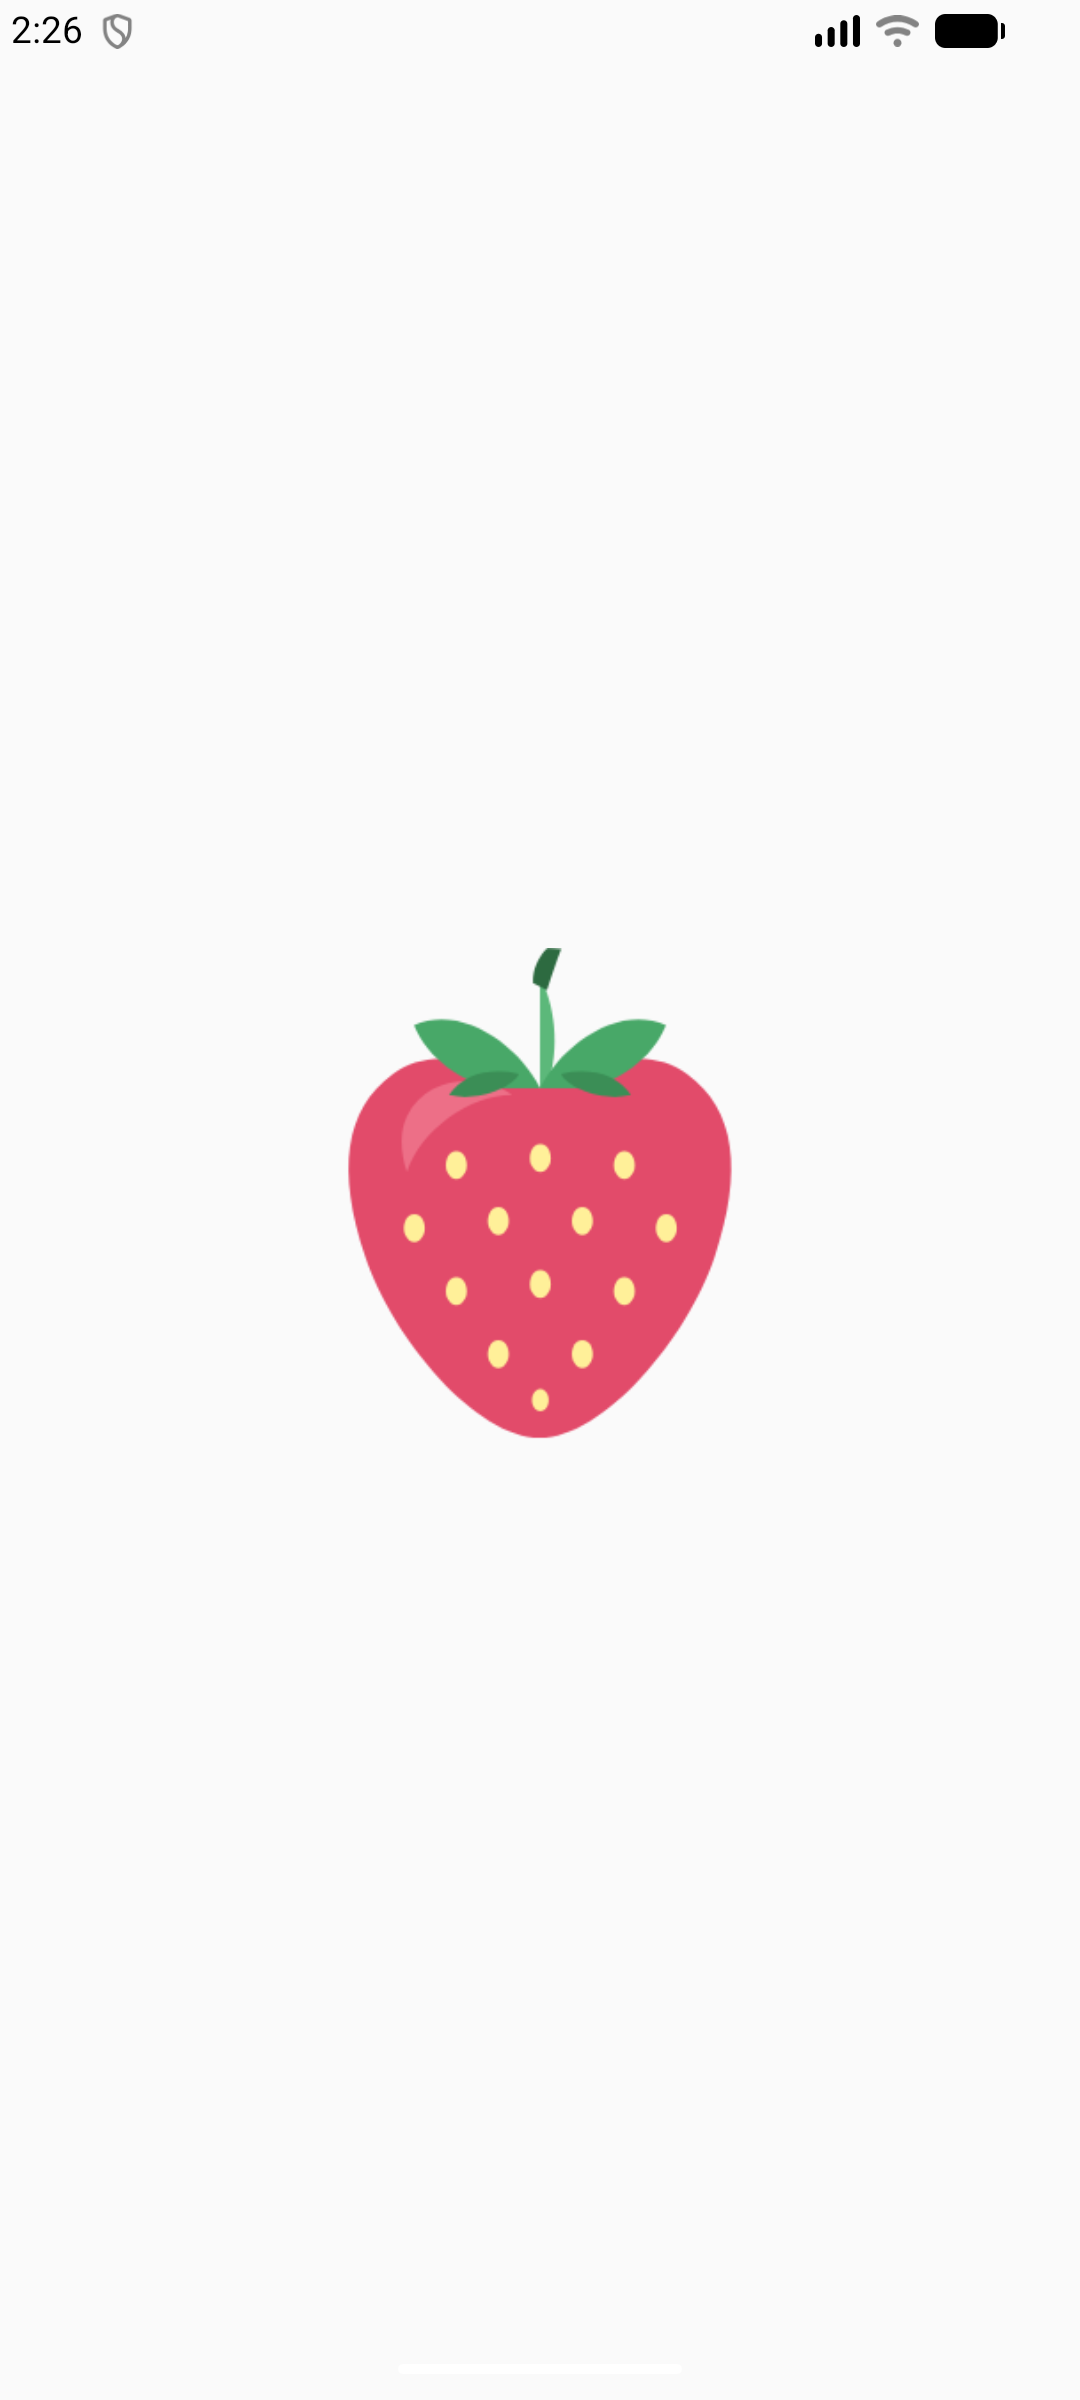
\includegraphics[width=0.48\textwidth]{images/screen_optimized_home.png}
    \caption{Schermata Home di SIMO 2.0: reattivit\`a dello stato Compose con warm-up asincrono immediato.}
    \label{fig:arch_home}
\end{figure}

\subsection{Struttura a Livelli (Layered Architecture)}
\begin{itemize}[leftmargin=*]
    \item \textbf{Presentation Layer (UI Declarative):} Composable modulari (`RecipeListScreen`, `RecipeDetailScreen`, `RecipeEditScreen`, `CookingModeScreen`, `ShoppingListScreen`), gestiti da StateFlow immutabili emessi dai ViewModel.
    \item \textbf{Domain Layer (Business Logic pura):} Modulo indipendente privo di dipendenze verso Android SDK:
    \begin{itemize}[noitemsep]
        \item `MathEngine`: Espansione DAG, scaling, reverse scaling, concentrazione nutrizionale, food cost;
        \item `RecipeTags`: Normalizzazione delle categorie e gestione di \textit{Panini};
        \item `ItalianGrammarUtils` e `CookingTimerExtractor`.
    \end{itemize}
    \item \textbf{Data Layer (Persistenza \& Cloud HAL):}
    \begin{itemize}[noitemsep]
        \item `AppDatabase`: Room SQLite ORM (Schema v12);
        \item `CryptoUtils`: AndroidKeyStore AES-256 GCM;
        \item `GeminiRecipeService` \& `OpenAiRecipeService`;
        \item `RecipePdfExporter` \& `BackupManager`.
    \end{itemize}
\end{itemize}

\subsection{Concorrenza e Thread Safety}
L'esecuzione \`e rigorosamente segregata sui dispatcher Kotlin:
\begin{itemize}[leftmargin=*]
    \item `Dispatchers.Main`: Binding reattivo Compose a 60 FPS;
    \item `Dispatchers.Default`: Attraversamento grafo DAG, calcolo nutrizionale e bilanciamento dosi;
    \item `Dispatchers.IO`: Query Room SQLite, I/O crittografico, client HTTPS REST e serializzazione PDF/JSON.
\end{itemize}

\newpage

% ==============================================================================
% SEZIONE 3: DOMAIN ENGINE - DAG, NUTRIZIONE E FOOD COST
% ==============================================================================
\section{Domain Engine: Teoria dei Grafi, Nutrizione e Calcolo Matematico}

\subsection{Formalizzazione del Ricettario come DAG Pesato}
Sia $G = (V, E, W)$ un grafo orientato pesato finito privo di cicli:
\begin{equation}
\forall v \in V, \quad \nexists \text{ cammino orientato } v \rightsquigarrow v \iff G \text{ \`e un DAG}
\end{equation}
dove $V = V_{\text{raw}} \cup V_{\text{recipe}}$ e $E \subseteq V_{\text{recipe}} \times V$.
Il peso dell'arco modella la quantit\`a base $q$ e l'unit\`a $u$.

\subsection{Algoritmo di Rilevamento Cicli Preventivo (\texttt{wouldCreateCycle})}
Prima di inserire o modificare un arco candidato $(u, v)$, il sistema esegue una BFS:
\begin{equation}
\text{hasCycle}(u, v) \iff u \text{ \`e raggiungibile da } v \text{ in } G
\end{equation}

\subsection{Modello Matematico dei Valori Nutrizionali e Concentrazione in Cottura}
Ciascun ingrediente base $i \in V_{\text{raw}}$ \`e caratterizzato da un vettore nutrizionale per 100\,g di materia prima cruda:
\begin{equation}
\vec{N}_i = \begin{pmatrix} C_i \\ K_i \\ F_i \\ P_i \\ W_i \\ S_i \end{pmatrix} = \begin{pmatrix} \text{Calorie [kcal]} \\ \text{Carboidrati [g]} \\ \text{Grassi [g]} \\ \text{Proteine [g]} \\ \text{Acqua [g]} \\ \text{Sodio [mg]} \end{pmatrix}
\end{equation}

Dato un albero scalato con insieme di foglie $c \in \text{Foglie}(R)$, ciascuna avente massa scalata $m(c)$ (convertita in grammi con densit\`a unitaria per i millilitri), l'apporto assoluto del componente \`e:
\begin{equation}
\vec{N}_{\text{tot}}(c) = \frac{m(c)}{100} \cdot \vec{N}_{\text{item}(c)}
\end{equation}

La massa totale cruda $W_{\text{raw}}$ e la massa cotta finita $W_{\text{cooked}}$ sono definite da:
\begin{equation}
W_{\text{raw}} = \sum_{c \in \text{Foglie}} m(c)
\end{equation}
\begin{equation}
W_{\text{cooked}} = W_{\text{raw}} \cdot \left(1 + \frac{\gamma}{100}\right), \quad \text{con } \gamma = \text{cookingWeightModifier} \in (-100, +\infty)
\end{equation}

\begin{archbox}[Legge di Concentrazione dei Nutrienti in Cottura]
I valori nutrizionali medi per 100\,g di prodotto finito cotto sono calcolati normalizzando la somma assoluta dei nutrienti rispetto alla massa cotta effettiva:
\begin{equation}
\vec{N}_{100\text{g}} = \frac{\sum_{c \in \text{Foglie}} \vec{N}_{\text{tot}}(c)}{W_{\text{cooked}}} \times 100
\end{equation}
Se $\gamma < 0$ (es. evaporazione del 10\%), $W_{\text{cooked}} < W_{\text{raw}}$ e la densit\`a nutrizionale per 100\,g aumenta coerentemente con la realt\`a termodinamica.
I valori per porzione singola sono invece indipendenti dall'evaporazione dell'acqua:
\begin{equation}
\vec{N}_{\text{porzione}} = \frac{\sum_{c \in \text{Foglie}} \vec{N}_{\text{tot}}(c)}{Y_{\text{target}}}
\end{equation}
\end{archbox}

\subsubsection{Derivazione di Energia e Sale Equivalente}
In conformit\`a con il Regolamento UE 1169/2011:
\begin{equation}
\text{Energia [kJ]} = (K \times 17) + (P \times 17) + (F \times 37)
\end{equation}
\begin{equation}
\text{Sale Equivalente [g]} = \frac{S\text{ [mg]}}{1000} \times 2.5
\end{equation}

\subsection{Modello Analitico del Food Cost ed Equivalenza Culinaria}
Il costo elementare $C(c)$ del componente scalato $c$ con quantit\`a $q(c)$ e unit\`a $u_r$, dato un prezzo unitario $p$ con unit\`a commerciale $u_p$, applica l'operatore di conversione esteso con equivalenza culinaria 1:1 ($g \leftrightarrow ml$, $kg \leftrightarrow l$):
\begin{equation}
\mu(u_r, u_p) = 
\begin{cases}
1 & \text{se } u_r = u_p \text{ oppure } (u_r \in \{g, ml\} \land u_p \in \{g, ml\}) \\
10^{-3} & \text{se } u_r \in \{g, ml\} \land u_p \in \{kg, l\} \\
10^3 & \text{se } u_r \in \{kg, l\} \land u_p \in \{g, ml\} \\
\frac{\text{gramsPerUnit}}{1000} & \text{se } u_r \in \{\text{unit\`a, pz}\} \land u_p \in \{kg, l\} \\
\text{gramsPerUnit} & \text{se } u_r \in \{\text{unit\`a, pz}\} \land u_p \in \{g, ml\} \\
0 & \text{se } u_r = \text{q.b.}
\end{cases}
\end{equation}

\newpage

% ==============================================================================
% SEZIONE 4: STRATO DATI, ROOM DATABASE E PERSISTENZA
% ==============================================================================
\section{Strato Dati, Room Database e Persistenza Reattiva}

\subsection{Schema Relazionale Room (Versione 12)}
Il database relazionale locale adotta Android Room SQLite con migrazione incrementale:

\begin{table}[h!]
\centering
\small
\begin{tabularx}{\textwidth}{p{3.2cm}p{4.2cm}X}
\toprule
\textbf{Tabella} & \textbf{Colonne Chiave} & \textbf{Descrizione e Campi v2.0} \\
\midrule
\texttt{items} & \texttt{id, name, type, defaultUnit, pricePerUnit, allergens, nutrizione} & Include \texttt{caloriesKcal}, \texttt{carbohydratesG}, \texttt{fatsG}, \texttt{proteinsG}, \texttt{waterG}, \texttt{sodiumMg} (REAL). \\
\texttt{recipes} & \texttt{id, name, baseYield, yieldUnit, category, cookingModifier} & Include \texttt{cookingWeightModifier} (REAL NOT NULL DEFAULT 0.0). \\
\texttt{recipe\_components} & \texttt{id, parentRecipeId, childItemId, baseQuantity, unit} & Modella gli archi orientati pesati del grafo DAG. \\
\texttt{shopping\_items} & \texttt{id, itemName, quantity, unit, unitPrice, priceUnit} & Articoli della spesa con persistenza dei prezzi unitari. \\
\bottomrule
\end{tabularx}
\caption{Schema delle tabelle principali in Room Database (Schema Version 12).}
\end{table}

\subsection{Pattern di Modifica Reattiva ed Entit\`a Immutabili}
In `RecipeEditViewModel.kt`, lo stato di modifica \`e incapsulato nella struttura immutabile `EditableComponent`:
\begin{lstlisting}[language=Kotlin]
data class EditableComponent(
    val tempId: String = UUID.randomUUID().toString(),
    val itemId: String,
    val itemName: String,
    val itemType: ItemType,
    val quantity: String,
    val unit: String,
    val pricePerUnit: Double? = null,
    val priceUnit: String? = null,
    val allergens: List<Allergen> = emptyList(),
    val caloriesKcal: Double? = null,
    val carbohydratesG: Double? = null,
    val fatsG: Double? = null,
    val proteinsG: Double? = null,
    val waterG: Double? = null,
    val sodiumMg: Double? = null
)
\end{lstlisting}

\newpage

% ==============================================================================
% SEZIONE 5: CLOUD AI ENGINE - GEMINI & CHATGPT
% ==============================================================================
\section{Integrazione Cloud AI: Dual-Engine Google Gemini \& OpenAI ChatGPT}

SIMO 2.0 offre un'architettura modulare bivalente per l'assistenza culinaria generativa (`GeminiRecipeService.kt` e `OpenAiRecipeService.kt`), gestita dall'enum `AiProvider`.

\subsection{Preservazione Intelligente dell'Unit\`a di Resa (\texttt{yieldUnit})}
Nel caso in cui l'utente indichi un'unit\`a di misura personalizzata della resa (es. \textit{torta}, \textit{bicchieri}, \textit{panini}, \textit{fette}, \textit{crostate}), il prompt di sistema vincola il modello mediante validazione gastronomica:
\begin{lstlisting}[language=Kotlin]
val userUnit = yieldUnit?.trim()?.takeIf{ it.isNotBlank() } ?: "porzioni"
val prompt = buildString{
    append("Resa base e Unita richiesta: $userYieldNum $userUnit.\n")
    append("""
        IMPORTANTE SULL'UNITA DELLA RESA ('yieldUnit'):
        L'utente ha impostato come unita di misura: "$userUnit".
        - Se "$userUnit" ha senso culinario per la ricetta (es. 'torta' per un dolce, 'bicchieri' per una bevanda, 'panini' per burger), DEVI MANTENERE "$userUnit" nel campo 'yieldUnit' e calibrare le dosi per essa.
        - Se invece "$userUnit" non ha senso (es. 'bicchieri' per pasta o pizza), imposta 'yieldUnit' a "porzioni".
    """.trimIndent())
}
\end{lstlisting}

\subsection{Metodi Operativi Non-Distruttivi in ViewModel}
\begin{itemize}[leftmargin=*]
    \item `applyNutritionalValuesOnly`: Arricchisce i 6 parametri nutrizionali delle materie prime esistenti senza alterare quantit\`a pesate, costi o allergeni precedentemente inseriti;
    \item `applyCompletedMissingIngredients`: Completa esclusivamente gli ingredienti con quantit\`a indefinita o zero, lasciando inalterati gli altri elementi dell'impasto;
    \item `generateFullRecipe`: Genera l'intera composizione della ricetta da zero.
\end{itemize}

\subsection{Sicurezza Hardware-Backed AES-256 GCM}
Le chiavi API di entrambi i provider sono memorizzate nel coprocessore hardware `AndroidKeyStore` mediante algoritmo AES-256 in modalit\`a GCM:
\begin{equation}
\text{Ciphertext} = \text{AES-GCM-256}_{K_{\text{hardware}}}(\text{API Key})
\end{equation}
La master key non pu\`o mai essere estratta dal chip crittografico, prevenendo qualsiasi compromissione in fase di backup o memoria di processo.

\newpage

% ==============================================================================
% SEZIONE 6: RENDERING GRAFICO E GENERATORE PDF A4 MULTIPAGINA
% ==============================================================================
\section{Rendering Grafico e Generazione PDF Multipagina}

L'esportazione documentale in formato A4 (72 DPI, $595 \times 842\,\text{pt}$) \`e implementata in `RecipePdfExporter.kt` mediante la pipeline vettoriale nativa `android.graphics.pdf.PdfDocument`.

\subsection{Partizione Semantica a Minimo 2 Pagine Garantite}
Per garantire il massimo rigore visivo e conformit\`a con gli standard di produzione:
\begin{itemize}[leftmargin=*]
    \item \textbf{Pagina 1 (Cruscotto Dati \& Specifiche):}
    \begin{itemize}[noitemsep]
        \item Intestazione SIMO con data di calcolo e resa target;
        \item Titolo della ricetta, categoria e Food Cost (totale e a porzione);
        \item Tabella sinottica degli ingredienti con dosi scalate ed etichettatura sotto-ricette;
        \item Riquadro evidenziato con i 14 allergeni normativi UE;
        \item Tabella completa della \textbf{Dichiarazione Nutrizionale UE} (per 100\,g e per porzione cotta finita).
    \end{itemize}
    \item \textbf{Pagina 2 (e successive):}
    \begin{itemize}[noitemsep]
        \item Avvio forzato di una nuova pagina con `startNewPage()`;
        \item Intestazione mini con titolo ricetta e numero di pagina;
        \item Sezione \textbf{PROCEDIMENTO DI PREPARAZIONE} con passaggi numerati, word-wrapping automatico e testo renderizzato in \textbf{nero solido (`Color.BLACK`)} ad alto contrasto, eliminando qualsiasi opacit\`a o sbiadimento ereditato dai divisori.
    \end{itemize}
\end{itemize}

\newpage

% ==============================================================================
% SEZIONE 7: SOTTOSISTEMA DI BACKUP E SERIALIZZAZIONE
% ==============================================================================
\section{Sottosistema di Backup, Serializzazione JSON e Risoluzione Conflitti}

\subsection{Specifica Canonica SIMO JSON Schema v2}
La struttura di esportazione in formato JSON v2 supporta la persistenza completa di tutti i dati introdotti nella nuova versione:
\begin{lstlisting}[language=Kotlin]
{
  "version": 2,
  "appName": "SIMO",
  "timestamp": 1774028400000,
  "items": [
    {
      "id": "ing_farina_00",
      "name": "Farina 00",
      "type": "RAW_INGREDIENT",
      "defaultUnit": "g",
      "pricePerUnit": 1.20,
      "priceUnit": "kg",
      "allergens": "GLUTINE",
      "caloriesKcal": 364.0,
      "carbohydratesG": 76.3,
      "fatsG": 1.0,
      "proteinsG": 10.3,
      "waterG": 14.0,
      "sodiumMg": 2.0
    }
  ],
  "recipes": [
    {
      "id": "recipe_pizza_margherita",
      "name": "Pizza Margherita",
      "baseYieldQuantity": 1.0,
      "yieldUnit": "pizza",
      "category": "Pizze",
      "cookingWeightModifier": -10.0,
      "instructions": "1. ...",
      "components": [ ... ]
    }
  ]
}
\end{lstlisting}

\subsection{Retro-Compatibilit\`a con Backup v1}
Il motore `BackupManager.kt` riconosce automaticamente la versione del documento: se viene importato un file con schema versione 1 privo di coordinate nutrizionali, i campi vengono inizializzati a `null` e `cookingWeightModifier` viene impostato sul default neutro `0.0`, prevenendo eccezioni di deserializzazione.

\newpage

% ==============================================================================
% SEZIONE 8: TESTING, VALIDAZIONE E QUALIT\`A DEL CODICE
% ==============================================================================
\section{Testing, Validazione e Qualit\`a del Codice}

La qualit\`a e l'integrit\`a matematica di SIMO 2.0 sono garantite da una suite estesa di \textbf{59 test unitari automatizzati} eseguiti su host JVM:

\begin{table}[h!]
\centering
\small
\begin{tabularx}{\textwidth}{llX}
\toprule
\textbf{Suite di Test} & \textbf{N. Test} & \textbf{Obiettivo di Validazione} \\
\midrule
\texttt{NutritionMathEngineTest} & 6 test & Calcolo nutrizionale ricorsivo, concentrazione nutrienti con calo peso, resa cotta, energia kJ/kcal e sale da sodio. \\
\texttt{NutritionDatabaseAndBackupTest} & 5 test & Persistenza Room dei 6 nutrienti, migrazione schema, serializzazione e ripristino JSON v2. \\
\texttt{NutritionDefaultRecipesAndPdfTest} & 4 test & Validazione nutrizionale delle 3 ricette di default (Cornetto, Crema, Pizza) e test impaginazione PDF. \\
\texttt{RecipeTagsTest} & 3 test & Categoria predefinita \textit{Panini}, ordinamento alfabetico dei tag e sanitizzazione case-insensitive. \\
\texttt{OpenAiRecipeServiceTest} & 4 test & Fallback modelli ChatGPT, parsing JSON nutrizionale, preservazione unit\`a custom (\textit{bicchieri}). \\
\texttt{GeminiRecipeServiceTest} & 4 test & Parsing JSON Gemini, mappatura flessibile allergeni, preservazione unit\`a di resa. \\
\texttt{MathEngineTest} & 13 test & Scaling proporzionale lineare, reverse scaling, calcolo food cost ed equivalenza 1:1 g/ml e kg/l. \\
\texttt{MathEngineSafetyTest} & 4 test & Robustezza a valori non finiti ($NaN, +\infty$), divisioni per zero e aciclicit\`a DAG. \\
\texttt{AllergenLogicTest} & 3 test & Riconoscimento 14 allergeni normativi UE ed ereditariet\`a ricorsiva. \\
\texttt{ItalianGrammarUtilsTest} & 8 test & Flessione singolare/plurale per etichette ricetta, unit\`a di misura e costi. \\
\texttt{ShoppingListLogicTest} & 3 test & Aggregazione ingredienti con stessa unit\`a, somme ponderate e stima spesa. \\
\texttt{CookingTimerExtractorTest} & 2 test & Riconoscimento regex dei timer di cottura e durate composte. \\
\bottomrule
\end{tabularx}
\caption{Riepilogo delle 12 suite di test automatizzate in SIMO 2.0 (59 test complessivi).}
\end{table}

\section{Conclusioni e Sintesi della Release 2.0}
L'architettura SIMO 2.0 consolida il motore di calcolo proporzionale introducendo la fisica termica della cottura (\textit{cooking weight modifier}), la conformit\`a al Regolamento UE 1169/2011 per le etichette nutrizionali, il supporto bivalente AI (Gemini \& OpenAI) con preservazione semantica dell'unit\`a di resa, la nuova categoria \textit{Panini} e la generazione documentale A4 multipagina con contrasto assoluto.

\end{document}
